\documentclass[aagreenthesis]{subfiles}
%\usepackage{macros}
\begin{document}
\chapter{Metrology Applications of Fluid Crystals}
\section{Experimental Design}

We created freely-suspended
smectic films with racetrack geometry, as shown in Fig.~\ref{fig:geometry},  using $8$CB ($4$-$n$-octylcyanobiphenyl), a fluid
smectic~A  liquid crystal  at room temperature that can be drawn into molecularly thin films freely suspended in
air~\cite{YoungLightScatteringStudyTwoDimensional1978,RosenblattFreelySuspendedFerroelectric1979,PindakTwodimensionalsystems1982}.
A mechanical drawing of the film holder is in the Supplemental Information.
%
\begin{figure}[H]
\centering
\includegraphics[keepaspectratio=true,width=.6\textwidth]{./figs/racetrack/intro/Figure1.pdf}
\caption{Smectic film flow meter geometry. (a) A stainless steel film holder
    (\SI{45.2}{\milli\metre} $\times$ \SI{34.8}{\milli\metre} $\times$ \SI{7.6}{mm})
    % is mounted on a black substrate, and
    has a $w=\SI{3.1}{\milli\metre}$-wide channel in the form of a racetrack cut to a
    depth $h=\SI{3.7}{\milli\metre}$. At
    viewing ports centered along each `arm', the channel is cut all the way through the film holder
    (a depth of $\SI{7.6}{\milli\metre}$). Gas is coupled into and out of the system by
    means of co-linear, \SI{2}{\milli\metre}-diameter holes at the ends of the film holder. Smectic films are created by
    coating the bottom of a glass coverslip (the spreader) with liquid crystal material and
    drawing it across the top opening of the channel.
    The film is shielded from random air currents from above by a sealed cover (not shown).
    The photomicrograph shows
    typical islands (localized regions with more layers than the background film) used to track flow of the film in one of the viewing regions of the racetrack. (b) Schematic cross-section of
    a smectic film suspended across the channel (not to scale). The film
    comprises an integer number of smectic layers and can be as thin as two
    molecules ($\sim 6$~nm).  In general, a meniscus forms where the film contacts
    the edges of the channel.}
\label{fig:geometry}
\end{figure}

Freely-suspended films are ideal flow sensors for several reasons. Because they are so thin, they extract very
little energy from the gas jet being measured. A comparison of the effective
areal densities in our system assuming mass densities
$\rho_\text{LC}=\SI{1.008e3}{kg/m^3}$ and $\rho_\text{air} = \SI{1.225}{kg/m^3}$, and
thicknesses $\SI{6}{nm}$ and $\SI{1}{\centi\metre}$ of the LC film and of the
layer of air in the channel respectively, shows that the mass per unit area of
the film is about $2000$ times smaller than that of the air it is measuring,
implying that smectic films should be very sensitive to the velocity of air
flowing over them. Smectic films are intrinsically much more stable than films
of conventional fluids, lasting up to several years in the laboratory, and have been used previously to probe $2$D hydrodynamics~\cite{QiMutualDiffusionInclusions2014,KuriabovaHydrodynamicinteractionsfreely2016} and
rheology~\cite{QiActivemicrorheologysmectic2017}, shear-stress
measurements~\cite{Parmarnovelboundarylayer1991}, and in pressure
metrology~\cite{ParmarPressuresensorusing1994,YablonskiiPressuresensorbased2002}.
The application described here uses smectic films for flow
measurements.

When a film is first drawn, it is typically only a few smectic layers thick and appears uniformly black in reflected light. In the prototype racetrack geometry sketched in Fig.~\ref{fig:geometry}(a), air is then injected at a known
volumetric flow rate into the continuous rectangular channel located beneath the film. The inlet airflow is
independently  monitored using a  mass airflow sensor (Honeywell AWM5101VN) capable of measuring flow rates between $0$
and $5$ standard litres per minute (SLPM). As the air flows through the channel, it shear couples to the liquid crystal,
causing circulation of the film around the racetrack. This flow typically pulls
some additional LC material in from the meniscus,
leading to the formation of small, disc-like islands embedded in the film. Since the reflectance of thin, freely-suspended films depends quadratically on thickness\cite{RosenblattOpticaldeterminationsmectic1980}, the islands are brighter than the background film and can easily be visualized using video microscopy. The motion of the islands is observed on the ``backstretch'' of the racetrack using a $5\times$ objective and
captured using a high-speed video camera (Vision Research Phantom v12.1) at rates of \numrange[range-phrase=--]{100}{5000} frames per second. The islands are tracked using the open source
Python library Trackpy~\cite{AllantrackpyTrackpyv02018}, allowing us to use PTV
methods~\cite{DracosParticleTrackingVelocimetry1996,Adamczyk2Dimensionalparticletracking1988, AdrianParticleImageVelocimetry2011, RaffelParticleImageVelocimetry2018} to measure the velocity field of the
film in the region of interest.

The device works by
optically measuring the island velocity, which
should be linearly coupled to the velocity of the airflow.
In contrast to other mechanical flow meters, our
flow meter should thus be uniformly sensitive to airflow, regardless of the airflow velocity.


Our experimental approach has much in common with traditional PTV methods, where tracer
particles are injected into the gas being measured and a light sheet created
by a laser is used to define an illuminated plane, so that the tracer particles
intersecting this plane can be tracked with a camera, mapping out the gas
flow.
A key difference is that our tracer particles (the islands) are embedded in a
fluid with low
vapor pressure ($< 10^{-6}$ torr)\cite{Deschamps2008} that couples hydrodynamically to the gas flow,
rather than relying on solid particles introduced into the gas. In the LC flow meter, the
gas thus remains free of foreign tracer particles, making this a useful, non-invasive  approach for systems where maintaining
gas purity is important.


\section{Theory and Simulation}

In order to act as an ideal mechanical flow meter, the LC device should couple linearly to the gas flow (i.e., with a sensitivity
independent of flow velocity) while having a minimal effect on the system being measured.

Linearity is an intrinsic feature of this system because of the standard no-slip
boundary condition between two fluids in contact.
Because the velocity of the air varies over the height
of the channel, the average air and film velocities will be slightly different.

In order to model the behavior of the LC flow meter, we first consider
two-phase, stratified flow in an infinitely long, rectangular pipe with symmetry about the
midplane, a geometry that is amenable to an analytic
approach~\cite{GovierFlowComplexMixtures2008,HuhUseAirLiquidTwoPhase2002}.



\begin{figure}[h!]
\centering
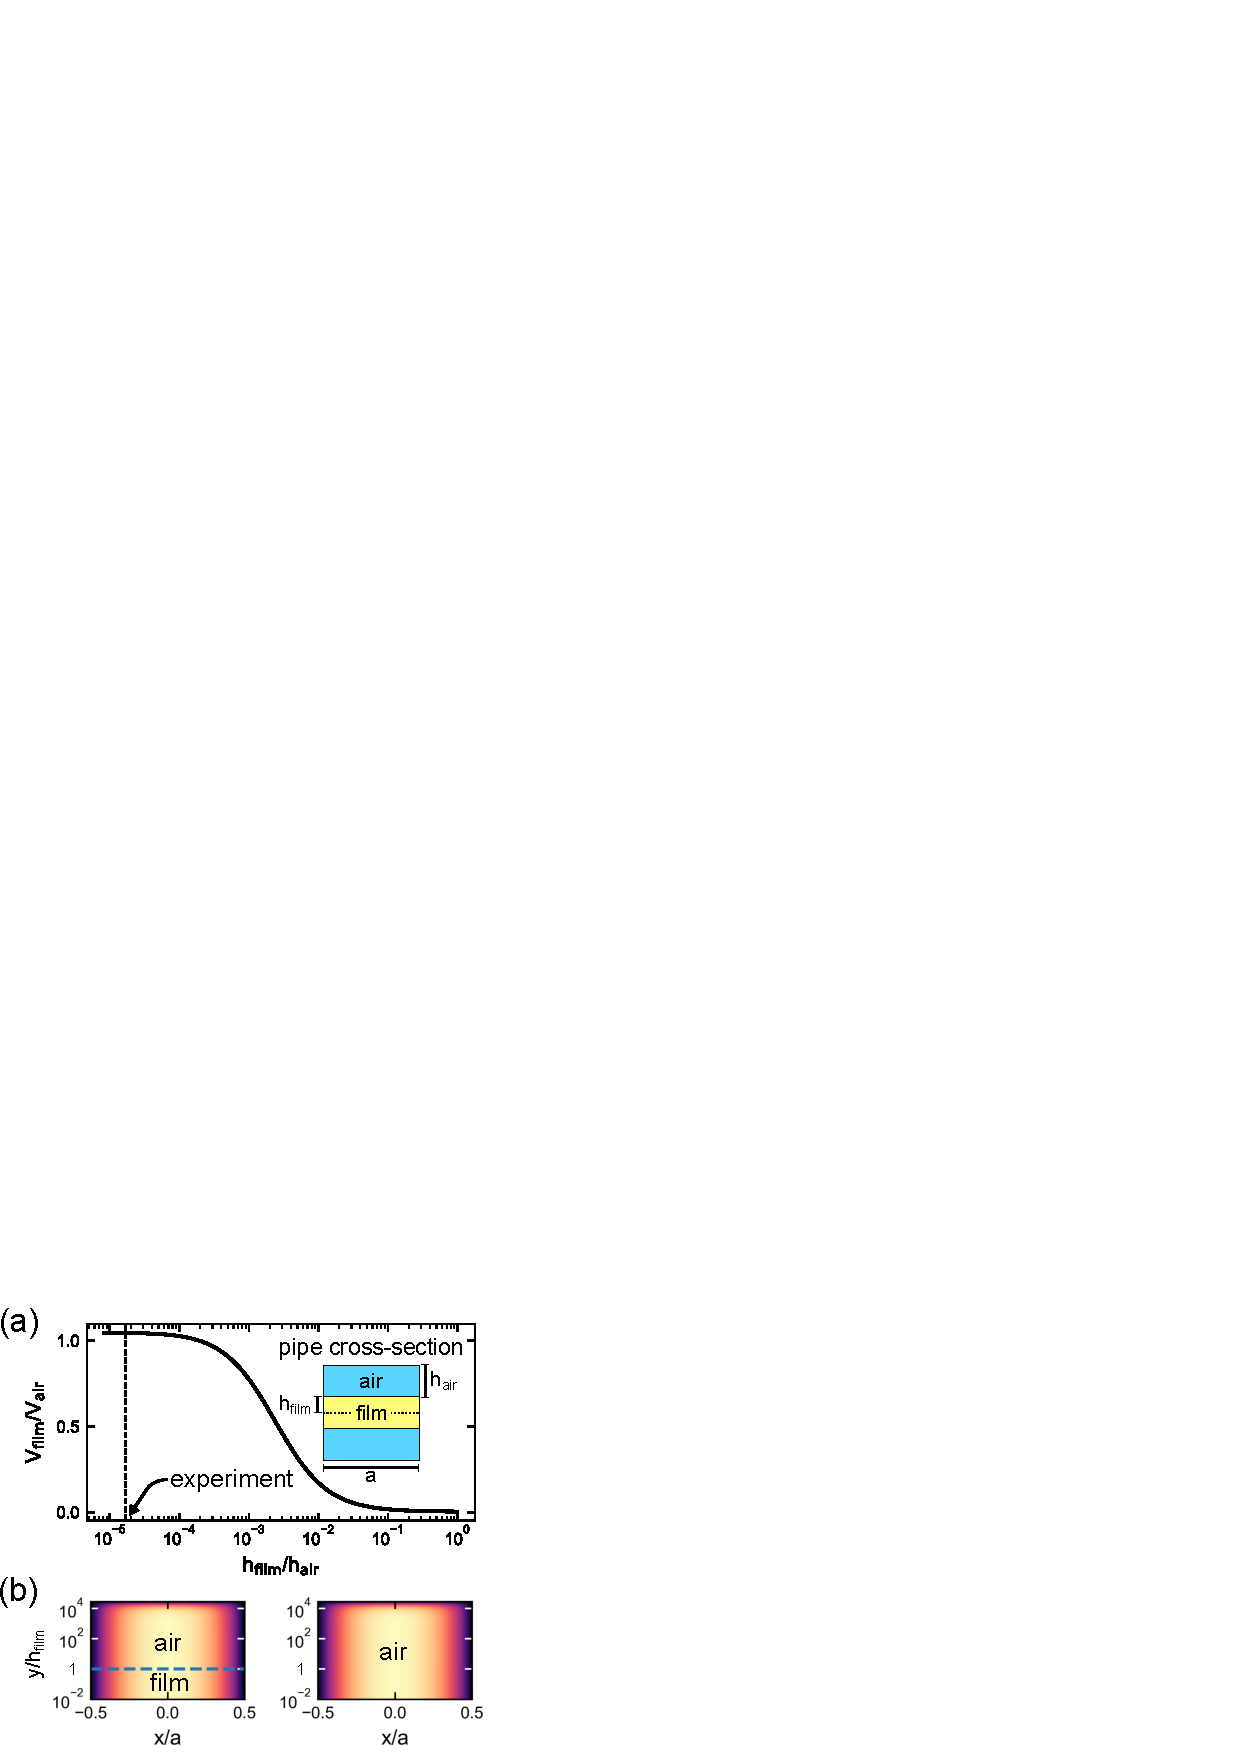
\includegraphics[keepaspectratio=true,width=.6\textwidth]{./figs/racetrack/theory/theory-final.pdf}
    \caption{Analytic analysis of symmetric, two-phase, stratified fluid flow in an infinitely long
    pipe of width $a$. (a) Ratio between the average film and air
    velocities as a function of the phase fraction (the ratio of the volume of the
    fluid and the volume of the air, $\phi=h_\text{film}/h_\text{air}$). When
    the phase fraction is very small, the film is strongly
    coupled to the air and moves with the same speed. (b) Flow velocity in the top half of the pipe. At left, both
    air and film are flowing through the pipe (the blue dashed line demarcates
    the upper boundary of the film), while on the right only air is present. The
    $y$ dimension is scaled by the half the thickness of the
    LC film, $h_\text{film}$. The flow fields in these two cases are practically indistinguishable, suggesting that the
    influence of the LC film on the airflow is negligible.
\label{fig:theory}}
\end{figure}

The symmetric rectangular pipe has the essential elements of the racetrack
flow meter, a multiphase system where a thin fluid is surrounded by air, but has
none of the complicating geometrical factors, allowing us to focus on the
intrinsic properties of the air and film interaction. By varying the relative
volume of the
air and liquid phases (the phase fraction), we can estimate the effect of a
fluid with the same thickness as a freely suspended film on the airflow.

We solved the Navier-Stokes equations to determine the airflow in the pipe both with and without the LC film,
using appropriate viscosities for
the air ($\SI{1.8e-5}{\pascal\second}$) and LC film
(\SI{5.2e-2}{\pascal \second})\cite{Schneider2006}. At
values of the phase fraction corresponding to the experiment (with a thick LC
film of 60 molecular layers, $\phi \sim 10^{-5}$),
the flow of the LC film is found to be coupled identically to that of the air  (Fig.~\ref{fig:theory}(a)).
Furthermore, the air flow in the presence of the LC film is essentially
indistinguishable from the flow in the absence of the film (Fig.~\ref{fig:theory}(b)), suggesting that, at least in
this idealized geometry, the film extracts a negligible amount of energy from
the air flow. Details of these calculations are given in the Supplemental
Information.

We numerically
modeled the flow of air in the 3D racetrack geometry, without the liquid crystal
film but choosing track dimensions and flow parameters consistent with our
experiments.

  Modeling the air flow alone allows us to see the
     ``natural state'' of flow in the racetrack geometry in the absence of the
     LC film. As the results of the analytical modeling in the previous section
     suggest that the film has a negligible influence on the airflow,
     we expect these airflow-only simulations to closely mimic the experimental
     behaviour. 
     
     The results of these simulations then allow us to see whether the
     geometry of the racetrack modifies the linear sensitivity predicted from
     the analytical model. We can also test the
     assumption that the film has a negligible impact on the overall flow
     behaviour by comparing the results of the air-flow simulations to the observed experimental flow behaviour. 

The simulations were performed using OpenFOAM, an open-source fluid dynamics
solver that uses a SIMPLE
algorithm\cite{Wellertensorialapproachcomputational1998}.
The results are summarized in Fig.~\ref{fig:simulation} with further details given in
the Supplemental Information.
The simulations indicate that at low inlet velocity values ($\lesssim
\SI[per-mode=symbol]{0.55}{\meter\per\second}$) the air stream in the channel splits, so that it flows
in the same absolute direction along both arms of the racetrack.
At $v_\text{in}=\SI[per-mode=symbol]{0.55}{\meter\per\second}$, the airflow is predicted to
transition to homogeneous, clockwise circulation.

The net force on an LC film in contact with the air stream is the sum of the shear forces along the entire
length of the racetrack, for which there are two main contributions:
the air moving along the shortest distance from the inlet to the
outlet (at speed $v_2$), and the air moving along the other side of the
racetrack (at speed $v_1$). Because the LC film is incompressible, if
$v_1$ and $v_2$ are in the same absolute direction, as in Fig.~\ref{fig:simulation}(a), then the steady
state film velocity is $v_\text{film}\propto v_2$-$v_1$.
This predicted film speed is in general lower than but roughly proportional to the inlet air flow, as shown in
Fig.~\ref{fig:simulation}(b).

We think that the chaotic
flow we observe in the racetrack is a manifestation of the `split-flow'
predicted by the simulations.  We hypothesize that the film
acts to bias the air-film system to a circulating regime, explaining why the air-film onset
to circulating flow happens at lower inlet velocities than the simulations predict
for pure airflow.



\begin{figure}[h!]
\centering
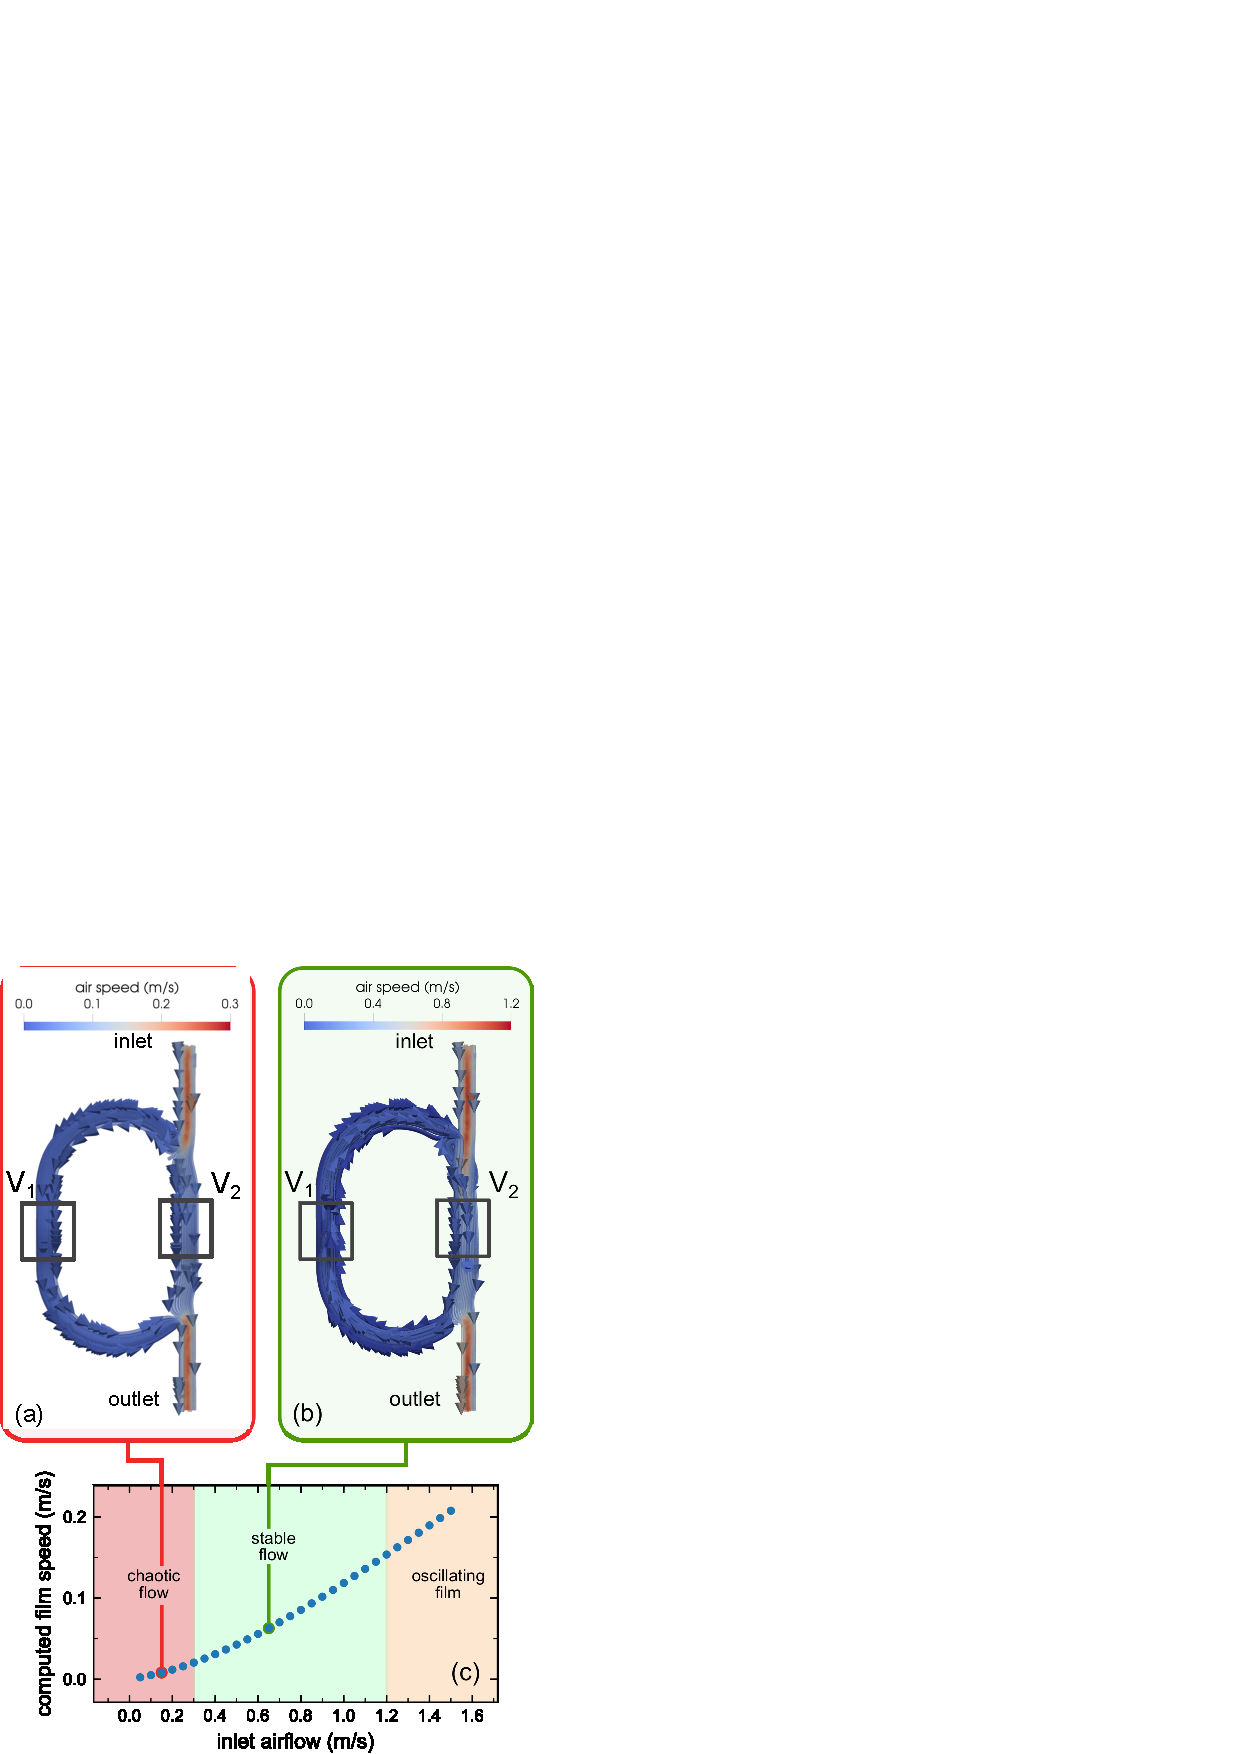
\includegraphics[keepaspectratio=true,width=.6\textwidth]{./figs/racetrack/simulation/simulation.pdf}
    \caption{Computed airflow in the racetrack geometry.
        (a) Model velocity field for inlet velocity $v_\text{inlet} =
        \SI[per-mode=symbol]{0.15}{\metre\per\second}$. The air does not circulate uniformly in the same sense around the racetrack,
    instead splitting between the front and back legs.
        (b) Model velocity field for inlet velocity $v_\text{inlet} =
        \SI[per-mode=symbol]{0.65}{\metre\per\second}$. Above a transition inlet velocity of
        $v_\text{inlet} = \SI[per-mode=symbol]{0.55}{\metre\per\second}$, the air circulates
        uniformly around the racetrack.
        (c) Predicted net film speed ($v_\textrm{film} \propto v_2-v_1$) for a
    range of inlet velocities. The slope of this curve gives an average theoretical sensitivity of
    $S= 0.15$. The background shading reflects the experimental
    observations with different inlet velocities: for  $v_\text{in} <
    \SI[per-mode=symbol]{0.3}{\metre\per\second}$, the film flow is chaotic; for
    $\SI[per-mode=symbol]{0.3}{\metre\per\second} < v_\text{in} <
    \SI[per-mode=symbol]{1.2}{\metre\per\second}$, the film exhibits stable
    Poiseuille flow; for $v_\text{in} > \SI[per-mode=symbol]{1.2}{\metre\per\second}$, the film
    undergoes rapid out-of-plane oscillations that make particle tracking
    impractical. \label{fig:simulation}}
\end{figure}

In summary, the analytic and numerical models both suggest that freely-suspended LC films in racetrack
geometry should make excellent flow detectors, linearly coupling to and stabilizing the air flow.


\section{Results and Discussion}
\begin{figure}
\centering
\includegraphics[keepaspectratio=true,width=.6\textwidth]{./figs/racetrack/bigfigure/mainresults.png}
\caption{Characterization of flow meter. (a) Velocity profiles over the width
    of the racetrack channel, with each point corresponding to a specific
    tracked island.
    The profiles are well described by parabolas (smooth curves), confirming Poiseuille flow over a
    wide-range of inlet velocities.
    At higher velocities, the data are noisier  due to the relatively paucity of islands that can be captured in sequential frames.
    The left-right asymmetry in the number of measurements is an artifact due to defects on one side of the camera sensor.
    (b) Spatially averaged film
    velocity in the observation region as a function of inlet air velocity. Measurements were performed over four
    separate days, using more than $30$ films. The volumetric flow rate of the
    air being injected into the racetrack through the inlet was measured using an independent
    mechanical sensor.
    The average film speed is linearly proportional to
    the speed of the air at the device inlet, with a sensitivity that is independent of flow rate.
    \label{fig:mainresults}}
\end{figure}



We measured the velocity
fields of LC films coupled to inlet airflows in the range
\SIrange[range-phrase=--]{0.1}{.4}{SLPM}. We observed three main regimes of film flow
behaviour, indicated by the shading in Fig.~\ref{fig:simulation}(c). Below a threshold inlet
air velocity ($v_\text{in} <
\SI[per-mode=symbol]{0.3}{\metre\per\second}$), the flow is characterized
by time-dependent, chaotic behavior, with flow reversal and eddy currents observed in the films.
This behavior is likely due to flow splitting of the type shown in Fig.~\ref{fig:simulation}(a), where the incoming air stream is divided
between the short and long arms of the racetrack.

At intermediate air inlet velocities
($\SI[per-mode=symbol]{0.3}{\metre\per\second}<v_\text{in} <
\SI[per-mode=symbol]{1.2}{\metre\per\second}$), the film undergoes uniform, counter-clockwise circulation around the racetrack,
as shown in Fig.~\ref{fig:mainresults}(a),
with a Poiseuille flow profile across the film that stabilizes in less than $1$
second.
The observed threshold speed for the transition from chaotic flow to uniform circulation
($v_\text{in} \sim \SI{0.3}{\metre\per\second}$) is somewhat lower than predicted by the simulations
for airflow alone ($v_\text{in} \sim \SI{0.55}{\metre\per\second}$).
This
suggests that the film acts to stabilize homogeneous flow,
promoting a uniform, regular circulation of the film and air. Because our
measurement relies on obtaining regular, simple flow, the stable regime is clearly optimal
for operation of the flow meter, and extending the usable range to lower inlet
velocities is a clear advantage of the LC film-air system. At high air inlet velocities
$(v_\text{in} > \SI[per-mode=symbol]{1.2}{\metre\per\second})$, the film
oscillates rapidly up and down, causing the islands to go in and out of focus and
the film eventually to break.


A comparison of the spatially averaged film speed measured half way along the
back stretch of the racetrack to the independently measured inlet airflow is plotted in
Fig.~\ref{fig:mainresults}(b). The average slope of this graph gives a measured
sensitivity of the flow meter of $S= 0.09$.
This is slightly less than the sensitivity predicted from the pure airflow
simulations, a difference which we attribute to air loss during the air-injection process.
With some refinement of the racetrack geometry, we would expect to extend the accessible measurement range to lower velocities.
The upper velocity limit could be raised by implementing measures to
equalize the air pressure across the film. We believe that such differences in air pressure
are responsible for the rapid vertical oscillations observed at high flow rates.


By harnessing the unique properties of freely-suspended smectic films, we have demonstrated a method for mechanical
measurement of air flow that has intrinsically linear sensitivity. This technique could usefully be applied to mapping
the velocity field of gases flowing through exotic microfluidic geometries in two dimensions.



\end{document}

